\section{TinyDAS}

In this section, we introduce TinyDAS, a Python program aimed at training autoencoder models and detecting anomalies within \acrshort{das} data. 

\subsection{Tools}

Tinygrad is a neural network framework created by George Hotz in October 2020 \cite{tinygrad2020}. It is based on Andrej Karpathys library \texttt{Micrograd} \cite{micrograd}, which aims to serve as an introduction to understand neural networks at its core. Tinygrad was introduced as an alternative to other popular frameworks such as \texttt{Pytorch} \cite{paszke2019pytorch} and \texttt{TensorFlow} \cite{abadi2016tensorflow}. The main goal is to \textquote{Build an equally performance stack to Pytorch on NVIDIA and AMD} \footnote{As stated in a conversation between George Hotz and Lex Friedman \cite{LexClipsYouTube2023}}. Unlike its alternatives, Tinygrad strives towards being hardware agnostic, where writing codes for different accelerators should be as similar as possible. For organizations, such as \acrshort{cgf} with limited hardware resources, this allows for an overall cheaper entry into scalable \acrshort{ml}, without sacrificing performance. \\

All operations in \texttt{Tinygrad} are lazy \cite{tinygrad}. This means that a binary operation tensors, such as $a+b$, is not computed until the \texttt{realize()} method is called. Additionally, \texttt{Tinygrad} strives to a more functional design pattern, with a limited amount of classes. Furthermore, \texttt{Tinygrad} has a built in \acrfull{jit} compiler, in which a kernel can be replayed, allowing for faster operations such as a \texttt{train} function. \\

For anomaly detection, we utilize several popular Python packages such as \texttt{numpy}, \texttt{scikit-learn} and \texttt{seaborn} for evaluation metrics, and \texttt{matplotlib} for visualization and plots. A full list of packages used can be found in 
appendix \ref{app:tinypacks}.


\subsection{Overview}
\label{meth:tinyoverview}

TinyDAS consists of two parts. The first part handles model construction and training, while the latter deals with anomaly detection of \acrshort{das} data. An overview of how TinyDAS works is shown in figure \ref{fig:dataflow}. The following list outlines the fundamental philosophies and criteria used to design and evaluate the framework:

\begin{figure}[!h]
    \centering
    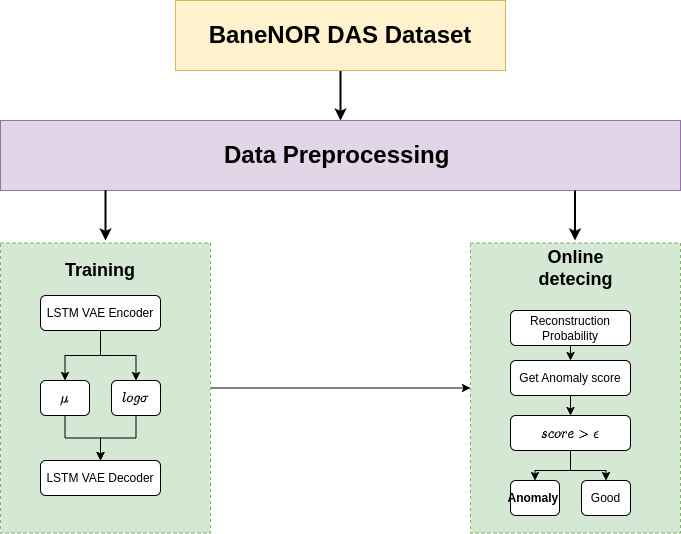
\includegraphics[scale=0.5]{figures/methodflow.png}
    \caption{Overview of TinyDAS}
    \label{fig:dataflow}
\end{figure}


\begin{enumerate}
    \item \textit{Support} for memory-efficient training techniques, specifically half-precision
    \item \textit{Scalability} from single-core systems to multi-node clusters
    \item \textit{Hardware agnostic} to ensure wide usability
    \item \textit{Modular architecture}, easily extendable with new models
    \item \textit{Separation of core logic} from data workflow for improved maintainability
    \item \textit{Collection} of different algorithms for anomaly detection
    \item \textit{Future potential} for online anomaly detection in a live environment
    \item \textit{Model-agnostic} approach to anomaly detection for broader applicability
\end{enumerate}

\subsection{Models} 

We implement four types of autoencoders: a linear autoencoder (AE), a convolutional autoencoder (CAE), a variational autoencoder ($\beta$-VAE), and a convolutional variational autoencoder ($\beta$-CVAE). The first model serves as a baseline against which to test. The latent space $Z$ can become disjoint and non-continuous in AE models, which $\beta$-VAE models try to solve. Additionally, we introduce convolutional layers in an attempt to improve the model's feature extraction capabilities. Based on this, these models serve as a baseline for what is to be expected by autoencoders for anomaly detection. Appendix \ref{app:archs} comprehensively describes layers and parameter sizes. \\

\subsection{\acrshort{api} design}

Due to Tinygrad being a relatively simple framework, we implement components to be used for training and testing, with the intent of being reusable and modular.

\subsubsection{Datasets and Dataloaders}

The \texttt{Dataset} and \texttt{DataLoader} classes support reading in \acrshort{hdf5} in batches, with support for data normalization and type casting. The former handles information about the dataset to be trained on and logic for loading a single file from a \acrshort{hdf5} file, or whatever other format might be sent in later on. The latter one handles the loading of batches in parallel, loading $n$ samples into the model.

\begin{figure}[!h]
    \centering
    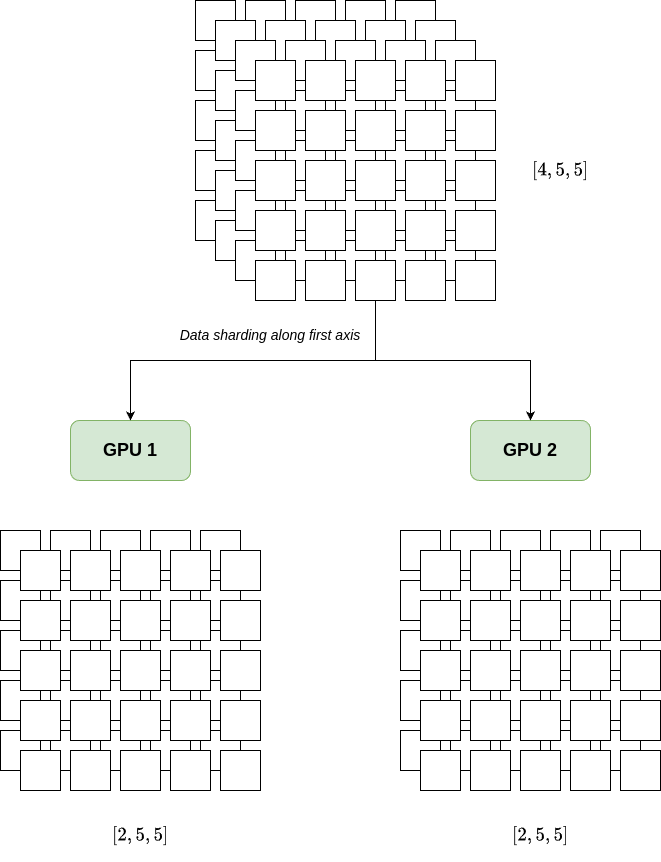
\includegraphics[width=0.5\linewidth]{figures/sharding.png}
    \caption{Example of data parallel training}
    \label{fig:dataparallel}
\end{figure}

\subsubsection{Autoencoder Base Class}

\lstinline{BaseAE} is the base model class from which all models are inherited. When training a model, the \lstinline{criterion} method is the main method to call. It runs the \lstinline{__call__} method and applies the loss function of choice. We define the class as follows:

\lstinputlisting[language=Python, label={lst:baseae}, caption=Base Autoencoder class]{code/baseae.py}

In addition to the methods shown in listing \ref{lst:baseae}, this class includes code for saving and loading, as well as different weight initialization methods such as \textit{He}- and \textit{Xavier} initialization \cite{kumar2017weight}.

\subsubsection{Trainer}

The Trainer class serves as the core component of our program. As demonstrated in listing \ref{fig:lstmcell}, it integrates a model, dataloader, and optimizer to execute the training process. Additionally, it handles early stopping, stores history of losses, and saves the best model for further use. The \texttt{Trainer} class is shown in code listing \ref{code:trainer} in the appendix. Note that the \texttt{@TinyJIT} macro enables kernel replays on subsequent calls, speeding up training and validation. 

\lstinputlisting[language=Python, caption=Core function snippets of the \texttt{Trainer} class, label={code:trainer}]{code/trainer.py}

One of the more important aspects of this class is the \texttt{train} function, which leverages the \acrshort{jit} compiler to replay this kernel for each iteration, resulting in faster training times. Furthermore, the \texttt{reshape\_fn} lambda function allows us to reshape data based on if our model is convolutional or not. For convoluional models, input should be $[BS, C, H, W]$ and $[BS, H, W]$ for models with linear input, where $BS$ is batch size, $C$ is amomunt of channels (always 1 for our \acrshort{das} data), and $H$ and $W$ is height and width of the matrix. This is not done in the model itself due to some instability with the \texttt{Tinygrad} \acrshort{api}. We continuously check and store the trainable parameters of the best performing models.


\subsection{Usage}

\subsubsection{Training}

In the same way that \texttt{Judas} is designed, we want \texttt{TinyDAS} to be modular and easy to use. We've designed components in a way that is familiar to that of \texttt{Pytorch}\cite{paszke2019pytorch}. Models can be trained using the following script:

\lstinputlisting[caption=Example of how models within \texttt{TinyDAS} is trained, language=Python]{code/tinydas_main.py}

TinyDAS supports training with \texttt{Float16} precision to optimize computational efficiency. This feature, which can be activated through configuration files, converts all weights and biases in the model to half-precision floating-point format, effectively reducing memory requirements by half.

For example, to initiate training of an autoencoder model using transfer learning on four \acrshort{gpu} devices, one would execute the following command:
\begin{lstlisting}[style=shellcommand, language=bash]
(*@\textcolor{promptcolor}{\$}@*) python main.py -m ae -t train -g 4 -l
\end{lstlisting}

where:
\begin{description}
\item[\texttt{-m ae}] specifies the autoencoder model
\item[\texttt{-t train}] sets the task to training
\item[\texttt{-g 4}] allocates four GPU devices
\item[\texttt{-l}] enables loading of a pre-trained model for transfer learning
\end{description}

This approach allows for flexible training of all TinyDAS models, accommodating various hardware configurations and leveraging pre-trained models through transfer learning. The model parameters are stored in the \texttt{safetensors} fileformat \cite{safetensors}.

\subsubsection{Hyperparameters and configurations}

Hyperparameters for the different models are stored in separate YAML files with the same name as the model. An example of a hyperparameter configuration can be found in appendix \ref{app:hyper}.


\subsubsection{Anomaly Detection}

After having trained the models on normal signal data, we move on to the anomaly detection section of our program. As mentioned in \ref{back:anomdet}, first decide which types of anomalies are to be found. We decided to first of all split the files into smaller files of \qty{5}{\si{\second}} files, partially to fascilitate for faster inference of our model. We decide to look at the whole array as whole, instead of finding segments. We will be calculating precisions, recalls and f1scores to find a threshold for reconstruction loss of our data to determine whether or not the data is anomalous. A function for finding this threshold is presented in code listing \ref{code:th}.  \\

\lstinputlisting[language=Python, caption=Code for finding the best threshold, label={code:th}]{code/bestth.py}

By finding the optimal threshold, we can utilize this in an online environment, preprocessing incoming \acrshort{das} data to fit our model and mark the data as anomalous if \lstinline[language=Julia]{reconstruction_error > threshold}. 

Clustering + LabelFree Detection for discussion? reconstruction error per cell and a clustering algorithm could find where in the signal the anomaly is found

